\documentclass{presentation}

\DeclareMathOperator\NOT{NOT}
\DeclareMathOperator\OR{OR}
\DeclareMathOperator\CSAT{CSAT}
\DeclareMathOperator\NP{\mathbf{NP}}
%\DeclareMathOperator\P{\mathbf{P}}
\renewcommand\P{\mathbf{P}}
\newcommand\COL{\mathrm{COL}}

\AtBeginDocument{
  \setlength\abovedisplayskip{0pt}
  \setlength\belowdisplayskip{0pt}
}

\definecolor{red}{HTML}{e00060}
\definecolor{green}{HTML}{f0b000}
\definecolor{blue}{HTML}{0050c0}

\tikzset{
  every picture/.style={
    circuit logic US
  },
  gates/.style={
    row sep=1em/2,
    column sep=2.5em,
  },
  vertex/.style={
    circle,
    draw,
    inner sep=0pt,
    minimum size=2em/3,
  },
  every matrix/.style={ampersand replacement=\&},
  every circuit symbol/.style={
    fill=lightgray,
    anchor=output,
  },
  input/.style={
  },
  output/.style={
  },
  pics/input full/.style 2 args={
    code={
      \begin{scope}[x=1em, y=1em]
        \filldraw[fill=lightgray]
        (-3/2,1) rectangle (0,-1);

        \begin{scope}[yscale=#1]
          \filldraw[fill=white]
          (-1/2,1/2) -- ++(135:1/2) -| ++(-1/2,-1/3) -- ++(-45:1/2) -- ++(0,-2/3) -| cycle;
          \filldraw[fill=lightgray, line join=bevel]
          (-1,1/6) -- ++(1/2,0) -- ++(135:1/2) edge +(0,1/3) -- +(-1/2,0);
        \end{scope}

        \node[below left, inner sep=1pt, color=gray!50!black, font=\scriptsize] at (0,1) {\(1\)};
        \node[above left, inner sep=1pt, color=gray!50!black, font=\scriptsize] at (0,-1) {\(0\)};

        \node[left] at (-3/2,0) {#2};
      \end{scope}
    },
  },
  pics/output glare/.style 2 args={
    code={
      \path[pic actions] ($ ({cos(#1)/2},{sin(#1)/4}) $) -- ++(0,1)
      arc[x radius=1/2*cos(#1), y radius=1/2-1/4*sin(#1), start angle=0, end angle=90]
      arc[x radius=1/2*cos(#2), y radius=1/2-1/4*sin(#2), start angle=90, end angle=0]
      -- ++(0,-1)
      arc[x radius=1/2, y radius=1/4, start angle=#2, end angle=#1];
    },
  },
  pics/output/.style n args={3}{
    code={
      \begin{scope}[x=1em, y=1em]
        \draw[wire, draw=#1] (0,0) -| (1/2,3/4);

        \pic[fill=#2, fill opacity=#3] at (1/2,3/4) {output glare={-180}{0}};
        \filldraw[fill opacity=1/4, draw opacity=1/2] (1/2,3/4) circle[x radius=1/2, y radius=1/4];
        \pic[fill=white, opacity=1/2] at (1/2,3/4) {output glare={-180}{-135}};
        \pic[fill=black, opacity=1/4] at (1/2,3/4) {output glare={0}{-60}};
        \pic[draw] at (1/2,3/4) {output glare={-180}{0}};

        %\fill[white, opacity=#3] (1/2,5/4) circle[radius=1/4];

        %\fill[opacity=1/4] (1,3/4) -- ++(0,1)
        %arc[radius=1/2, start angle=0, end angle=90]
        %arc[x radius=1/2*sin 30, y radius=1/2+1/4*cos 30, start angle=90, end angle=0]
        %-- ++(0,-1)
        %arc[x radius=1/2, y radius=1/4, start angle=-60, end angle=0];
      \end{scope}
    },
  },
  pics/output 0/.style={output={blue}{gray}{1/2}},
  pics/output 1/.style={output={red}{red}{1}},
  pics/input 1/.style={input full={1}{#1}},
  pics/input 0/.style={input full={-1}{#1}},
  joint/.style={
    circle,
    fill=black,
    inner sep=0pt,
    minimum size=1.5pt,
  },
  on/.style={
    red,
  },
  wire/.style={
    thick,
    rounded corners=1em/4,
    to path={
      -- ($ (\tikztostart)!1/4!(\tikztostart -| \tikztotarget) $)
      -- ($ (\tikztotarget)!1/4!(\tikztostart |- \tikztotarget) $)
      -- (\tikztotarget)
    },
  },
  wire 0/.style={wire, color=blue},
  wire 1/.style={wire, color=red},
  focus 0/.style={opacity=1/3},
  focus 1/.style={opacity=1},
  gate legend grid/.style={
    tiny circuit symbols,
    matrix of nodes,
    row sep=1em/2,
    nodes={anchor=west, inner sep=0pt},
    column sep=1em/2,
    fill=lightgray!50,
    inner xsep=1em/2,
  },
  gate legend/.pic={
    \matrix[gate legend grid, left]{
      |[not gate]| \& \(\NOT\) \& \draw[wire, color=blue](0,0) -- (1em,0); \& \(0\) \\
      |[or gate]| \& \(\OR\)   \& \draw[wire, color=red](0,0) -- (1em,0); \& \(1\) \\
    };
  },
  pics/csat/.style n args={3}{
    code={
      \pgfmathtruncatemacro\x{#1}
      \pgfmathtruncatemacro\y{#2}
      \pgfmathtruncatemacro\z{#3}

      \matrix[gates](gates){
        \coordinate[input](x); \& \coordinate(x'); \\
        \& \node[not gate](nx){}; \& \node[or gate](o1){}; \& \node[not gate](n1){};
        \& \node[or gate](o4){}; \& \coordinate[output](out);
        \& \coordinate[output](y); \\
        \coordinate[input](y);
        \& \node[not gate](ny){}; \& \node[or gate](o2){}; \& \node[not gate](n2){}; \\
        \& \node[or gate](o3){}; \\
        \coordinate[input](z); \\
      };

      \draw[wire \x] (x) to (x') to (o1.input 1) (x) to (nx.input);
      \draw[wire \y] (y) to (ny.input) (y) to (o3.input 1);
      \draw[wire \z] (z) to (o3.input 2);

      \pgfmathtruncatemacro\nx{not(\x)}
      \pgfmathtruncatemacro\ny{not(\y)}
      \draw[wire \nx] (nx.output) to (o2.input 1);
      \draw[wire \ny] (ny.output) to (o1.input 2);

      \pgfmathtruncatemacro\ooo{or(\y,\z)}
      \draw[wire \ooo] (o3.output) to (o2.input 2);

      \pgfmathtruncatemacro\o{or(\x,\ny)}
      \pgfmathtruncatemacro\oo{or(\nx,\ooo)}
      \draw[wire \o] (o1.output) to (n1.input);
      \draw[wire \oo] (o2.output) to (n2.input);

      \pgfmathtruncatemacro\n{not(\o)}
      \pgfmathtruncatemacro\nn{not(\oo)}
      \draw[wire \n] (n1.output) to (o4.input 1);
      \draw[wire \nn] (n2.output) to (o4.input 2);

      \pgfmathtruncatemacro\out{or(\n,\nn)}
      \draw[wire \out] (o4.output) to (out);

      \pic at (x) {input \x=\(x\)};
      \pic at (y) {input \y=\(y\)};
      \pic at (z) {input \z=\(z\)};

      \pic at (out) {output \out};

      %\node[left] at (x){\(x\)};
      %\node[left] at (y){\(y\)};
      %\node[left] at (z){\(z\)};

      \pic[above left] at (gates.south east) {gate legend};

    },
  },
  box inputs/.style={
    rounded corners=1em/4,
    opacity=1/2,
    ->,
  },
  pics/box inputs/.style 2 args={
    code={
      \draw[box inputs]
      ($ (#1) + (-2.75em,1.5em) $) coordinate (#1-nw)
      rectangle ($ (#2) + (.5em,-1.5em) $) coordinate (#2-se);
    },
  },
  pics/color base/.style n args={6}{
    code={
      \coordinate[vertex, fill=#6] (o) at (0,0);
      \coordinate[vertex, fill=#1] (v0) at (0/5*360:4em);
      \coordinate[vertex, fill=#2] (v1) at (1/5*360:4em);
      \coordinate[vertex, fill=#3] (v2) at (2/5*360:4em);
      \coordinate[vertex, fill=#4] (v3) at (3/5*360:4em);
      \coordinate[vertex, fill=#5] (v4) at (4/5*360:4em);
      \foreach \i in {0,...,4} { \draw (o) -- (v\i); }
    },
  },
  uncolorable 0/.pic={
    \pic{color base={white}{red}{blue}{white}{white}{white}};
    \draw (v0) -- (v1) -- (v2) -- (v3) -- (v4) -- (v0);
  },
  uncolorable 1/.pic={
    \pic{color base={blue!50}{red}{blue}{blue!50}{red!50}{green!50}};
    \draw (v0) -- (v1) -- (v2) -- (v3) -- (v4) -- (v0);
    \node[above left, inner sep=0pt] at (4em,-4em){no :(};
  },
  colorable 0/.pic={
    \pic{color base={white}{red}{blue}{white}{white}{white}};
    \draw (v0) -- (v1) -- (v2) -- (v3) (v4) -- (v0);
  },
  colorable 1/.pic={
    \pic{color base={blue}{red}{blue}{red}{red}{green}};
    \draw (v0) -- (v1) -- (v2) -- (v3) (v4) -- (v0);
  },
  outside/.style={
    densely dotted,
  },
  gadget not/.pic={
    \begin{scope}[x=3em, y=3em]
      \coordinate[vertex](in) at (-1/2,0);
      \coordinate[vertex](out) at (1/2,0);
      \coordinate[vertex, fill=green](g) at (0,-sqrt 3/2);
      \node[above] at (in.north) {in};
      \node[above] at (out.north) {out};
      \draw[thick] (in) -- (out) -- (g) -- (in);
      \draw[outside] (in) -- +(-1,0);
      \foreach \i in {0,...,3} {
        \draw[outside] (out) -- +(-30+20*\i:1);
      }
    \end{scope}
  },
  gadget or/.pic={
    \begin{scope}[x=3em, y=3em]
      \coordinate[vertex](x) at (-1,0);
      \coordinate[vertex](y) at (-1,-1);
      \coordinate[vertex](x') at (0,0);
      \coordinate[vertex](y') at (0,-1);
      \coordinate[vertex](out) at (-30:1);
      \coordinate[vertex, fill=green](g) at (-1,-1/2);
      \coordinate[vertex, fill=green](g') at (sqrt 3/2,-1);
      \node[above] at (x.north) {in};
      \node[below] at (y.south) {in};
      \node[above] at (out.north) {out};

      \draw[outside] (x) -- +(-1,0);
      \draw[outside] (y) -- +(-1,0);
      \foreach \i in {0,...,3} {
        \draw[outside] (out) -- +(-30+20*\i:1);
      }

      \draw[thick]
      (x) -- (x') -- (out)
      (y) -- (y') -- (out)
      (x') -- (y')
      (x) -- (g) -- (y)
      (out) -- (g');
    \end{scope}
  },
}

\title{You can solve it, but can you play it?}
\author{Kye Shi\\\textsc{\textcolor{gray!50!black}{advisor}} Nick Pippenger}
\date{2021 November 30}

\begin{document}

\begin{frame}
  \maketitle
\end{frame}

\begin{frame}
  \frametitle{Circuit basics}
  \vfill

  \begin{center}
    \begin{tikzpicture}
      \alt<2,3>{\pgfmathtruncatemacro{\x}{1}}{\pgfmathtruncatemacro{\x}{0}}
      \alt<3,4>{\pgfmathtruncatemacro{\y}{1}}{\pgfmathtruncatemacro{\y}{0}}

      \matrix[gates] {
        \coordinate[input](x); \& \node[not gate](not){}; \\
        \&\& \node[or gate](or){}; \& \coordinate[output](out); \\
        \coordinate[input](y); \& \coordinate(y'); \\
      };

      \pic at (x) {input \x};
      \pic at (y) {input \y};

      \pgfmathtruncatemacro{\nx}{not(\x)}
      \pgfmathtruncatemacro{\ny}{not(\y)}
      \pgfmathtruncatemacro{\o}{or(\nx,\y)}
      \draw[wire \x] (x) to (not.input);
      \draw[wire \nx] (not.output) to (or.input 1);
      \draw[wire \y] (y) to (y') to (or.input 2);
      \draw[wire \o] (or.output) to (out);

      \pic at (out) {output \o};

    \end{tikzpicture}

  \end{center}

  \vfill
  \raggedleft\tikz{\pic{gate legend}}

\end{frame}

\begin{frame}
  \frametitle{A ``trivial'' problem}
  \begin{center}
    \begin{tikzpicture}
      \alt<2>{}{
        \tikzset{
          wire 0/.style={wire, color=gray},
          wire 1/.style={wire, color=gray},
          pics/output 0/.style={output={gray}{gray}{1/2}},
          pics/output 1/.style={output={gray}{gray}{1/2}},
        }
      }
      \pic{csat=000};
    \end{tikzpicture}

    What is the value of the output?
  \end{center}

  \pause
  \begin{itemize}
    \item Easy: answer can be computed quickly (in polynomial time)!
  \end{itemize}
\end{frame}



\begin{frame}
  \frametitle{The circuit satisfiability \emph{puzzle} (\(\CSAT\))}
  \begin{center}
    \begin{tikzpicture}
      \alt<1>{\pic{csat=000}}{\pic{csat=100}};
    \end{tikzpicture}

    Is there an input combination that satisfies this circuit?
    \visible<2->{Yes!}

  \end{center}

  \visible<3->{
    How hard is \(\CSAT\)?
    \begin{itemize}[nosep]
      \item Not as easy: solution obtained by \emph{guess}-and-check
        \begin{itemize}[nosep]
          \item \(\{\text{guess-and-check-solvable problems (``puzzles'')}\} = \NP\)
        \end{itemize}
      \item Circuits can represent \emph{any} function \(\{0,1\}^m \to
        \{0,1\}^n\)
      \item \(\CSAT\) is a ``maximally hard'' problem in \(\NP\) (\(\NP\)-complete)
    \end{itemize}
  }

  %remarks: can compute any boolean function.  "complete", which means any
  %puzzle (solution can be obtained by guess-and-check) can be reduced to it.

\end{frame}

\begin{frame}
  \frametitle{The two-turn \emph{game} (\(\CSAT_2\))}
  \begin{center}
    \begin{tikzpicture}
      \only<1-2>{\pic{csat=100}};
      \only<3>{\pic{csat=101}};
      \only<4>{\pic{csat=011}};
      \only<5->{\pic{csat=010}};

      \visible<2->{
        \pic{box inputs=zz};
        \node[above right] (jon) at (z-se) {mine};
        %{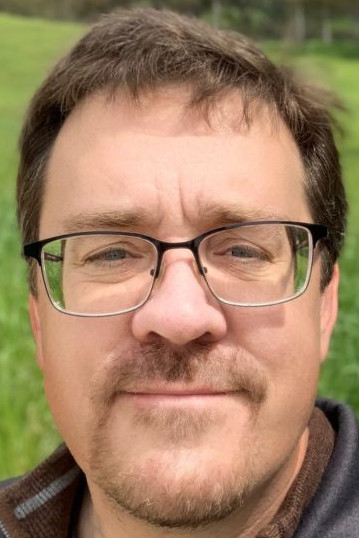
\includegraphics[width=2em, valign=m]{jj-crop.jpg}: \dots but these are mine.};
        %\draw[box inputs] (jon) -| ($ (z-se)!1/2!(z-se -| z-nw) $);

        \pic{box inputs=xy};
        %\node[right] (you) at ($ (x-nw -| y-se) + (2em,1em) $) {These are yours\dots};
        \node[below right] (you) at (x-nw -| y-se) {yours};
        %\draw[box inputs] (you) -| ($ (x-nw)!1/2!(x-nw -| y-se) $);
      }
    \end{tikzpicture}

    \visible<2->{
      If you go first, can you guarantee a win?  i.e.,
      \[
        [\exists x, y \quad \forall z \quad \operatorname{circuit}(x,y,z) = 1]?
      \]
    }
  \end{center}
  \visible<5->{
    How hard is \(\CSAT_2\)?
    \begin{itemize}[nosep]
      \item Probably harder than \(\CSAT_1\) (the puzzle)!
      \item \(\Sigma_2 \P\)-complete
    \end{itemize}
  }
\end{frame}

\begin{frame}
  \frametitle{\(n\)-turn \(\CSAT\) games}

  \begin{itemize}
    \item \(0\) turns: circuit checking (easy)
    \item \(1\) turn:\quad \(\exists X \; \operatorname{circuit}(X) = 1\)?
      (a.k.a., \(\CSAT\) the puzzle)
    \item \(2\) turns:\quad \(\exists X_1 \; \forall X_2 \;
      \operatorname{circuit}(X\dots) = 1\)?
    \item \(3\) turns:\quad \(\exists X_1 \; \forall X_2 \; \exists X_3 \;
      \operatorname{circuit}(X\dots) = 1\)?
    \item \(4\) turns:\quad \(\exists X_1 \; \forall X_2 \; \exists X_3 \;
      \forall X_4 \; \operatorname{circuit}(X\dots) = 1\)?
    \item[] \(\vdotswithin{\text{\(n\) turns}}\)
  \end{itemize}

  \[
    \underbrace{\CSAT_0}_{\P}
    \le \underbrace{\CSAT_1}_{\NP}
    \le \underbrace{\CSAT_2}_{\Sigma_2\P}
    \le \underbrace{\CSAT_3}_{\Sigma_3\P}
    {} \le \dotsb
  \]

\end{frame}

\begin{frame}
  \frametitle{Another puzzle: graph 3-coloring (\(3\COL\))}

  \begin{center}
    \begin{tikzpicture}
      \pgfmathtruncatemacro\step{0}
      \only<2->{\pgfmathtruncatemacro\step{1}}
      \matrix[column sep=4em]{
        \pic{uncolorable \step}; \& \pic{colorable \step}; \\
      };
    \end{tikzpicture}

    Can you color in the blank nodes with \(\{\tikz{\coordinate[vertex,
      fill=red]()}, \tikz{\coordinate[vertex, fill=green]()},
    \tikz{\coordinate[vertex, fill=blue]()}\}\) such that\\
    every pair of neighbors has distinct colors?

    \vfill

  \end{center}

  \visible<3->{
    How difficult is \(3\COL\)?
    \begin{itemize}[nosep]
      \item Guess-and-check solvable, so \(3\COL \le \CSAT_1\).
      \item \dots Can we say more?
        \begin{itemize}[nosep]
          \item \visible<4->{Yes! Claim: \(3\COL\) and \(\CSAT\) have the \emph{same} difficulty.}
        \end{itemize}
    \end{itemize}
  }

\end{frame}

\begin{frame}
  \frametitle{Claim: \(\CSAT \le 3\COL\)}

  Approach: given a circuit \(C\), convert it into a graph \(G\) so that
  \[
    \text{\(G\) is \ul{colorable}} \iff \text{\(C\) is \ul{satisfiable}}.
  \]

  Represent wires with nodes, \({\color{red}1} = \tikz{\coordinate[vertex,
  fill=red]()}, {\color{blue}0} = \tikz{\coordinate[vertex, fill=blue]()}\),
  and replace gates with:
  \begin{center}
    \begin{tikzpicture}
      \matrix[row sep=1em/2, column sep=4em]{
        \node{\(\NOT\)}; \& \node{\(\OR\)}; \\
        \pic{gadget not}; \& \pic{gadget or}; \\
      };
    \end{tikzpicture}
  \end{center}

  \vfill
  \pause
  \begin{itemize}[nosep]
    \item \(3\COL\) is \emph{equivalent to} \(\CSAT\)!
    \item Next up: \(3\COL\) \emph{games}!  \emph{More puzzles!}
  \end{itemize}
\end{frame}

\end{document}
